\section{实验步骤}
    \textbf{操作步骤+运行截图}
    \subsection{实验内容一}
        \subsubsection{代码解释}
            \subsubsection*{基础功能}
                \begin{enumerate}
                    \item 定义学生结构体,数据项包含学号、姓名、年龄。
                        \begin{figure*}[htbp]
                            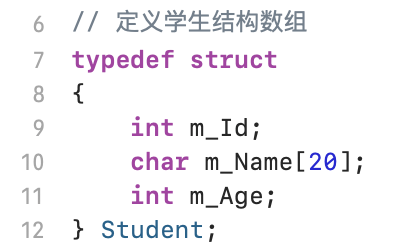
\includegraphics[width = 7cm]{work1_s1.png}
                        \end{figure*}
                    \item 将学生结构体封装进线性表,便于后续文件读写操作。
                        \begin{figure*}[htbp]
                            \includegraphics*[width = 15cm]{work1_s2.png}
                        \end{figure*}
                    \newpage
                    \item \textbf{\textit{init()}} 函数用于从 \textbf{\textit{input.dat}} 中读取数据初始化线性表,如果没有任何数据,则会将表长初始化为 \textbf{\textit{0}},否则将会读入历史数据。
                        \begin{figure*}[htbp]
                            \includegraphics*[width = 14cm]{work1_s3.png}
                        \end{figure*}
                \end{enumerate}
            \subsubsection*{功能项 1}
                \par 依次输入五名学生的信息,由于学号递增,只需输入第一位学生的学号。
                \par \textbf{\textit{index}} 可以表示表长,同时也表示指向表尾后一位的指针,这就代表我们可以通过 \textbf{\textit{index}} 向线性表中添加元素。
                \par 因此每次只要将学生添加到数组下标为 \textbf{\textit{index}} 的位置,并在一次迭代结束时令 \textbf{\textit{index ++ }},使其指向下一个位置。
                \begin{figure*}[htbp]
                    \includegraphics*[width = 17cm]{work1_s4.png}
                \end{figure*}
            \newpage
            \subsubsection*{功能项 2}
                \par 以二进制方式写入文件,如果文件无法打开,则抛出异常,否则将表长和学生结构体数组存入 \textbf{\textit{input.dat}} 中。
                \begin{figure*}[htbp]
                    \includegraphics*[width = 12cm]{work1_s5.png}
                \end{figure*}
            \subsubsection*{功能项 3}
                \par 由于我们需要将一个文件里的数据逆序写入到另一个文件中,所以需要创建一个临时的线性表接受数据,再将其逆序写入新的文件中。
                \par 在程序中,首先创建了临时变量 \textbf{\textit{temp}},并将 \textbf{\textit{input.dat}} 的数据读入 \textbf{\textit{temp}} 中,同时由于读入学生结构体数组时需要用到线性表的表长,因此先读入表长,这也是存储时先存储表长的原因。
                \par 在写入时,我们从数组下标为 \textbf{\textit{index - 1}} 处开始写入,以此实现逆序输出的要求。
                \begin{figure*}[htbp]
                    \includegraphics*[width = 11cm]{work1_s6.png}
                \end{figure*}
            \subsubsection*{附加要求}
                \par 具体实现见运行截图中的说明。
        \subsubsection{运行截图}
            \begin{enumerate}
                \item 在 \textbf{\textit{func1()}} 循环中设置条件断点。
                \begin{figure*}[htbp]
                    \centering
                    \includegraphics*[width = 10cm]{work1_s7.png}
                \end{figure*}
                \item 运行程序,可以看到,程序在执行到处理第 $5$ 位学生信息时中断。
                \begin{figure*}[htbp]
                    \centering
                    \includegraphics*[width = 10cm]{work1_s8.png}
                \end{figure*}
                \item 继续运行,程序结束
                \newpage
                \item 第二次运行程序,我们可以在监视栏看到上一次运行的数据被成功保存并读入进来。
                \begin{figure*}[htbp]
                    \centering
                    \includegraphics*[width = 10cm]{work1_s9.png}
                \end{figure*}
                \item 继续运行,发现由于 \textbf{\textit{index}} 的存在,使得程序可以正确地从上一次截止位置继续添加学生信息。
                \begin{figure*}[htbp]
                    \centering
                    \includegraphics*[width = 10cm]{work1_s10.png}
                \end{figure*}
                \newpage
                \item 第三次运行程序,我们修改 \textbf{\textit{init()}} 函数的参数,从 \textbf{\textit{output.dat}} 中读入数据,并输出。
                \begin{figure*}[htbp]
                    \centering
                    \includegraphics*[width = 10cm]{work1_s11.png}
                \end{figure*}
                \item 可以看到,输出的内容是逆序的,说明我们在上两次程序中成功将数据逆序存储到了 \textbf{\textit{output.dat}} 中。
                \begin{figure*}[htbp]
                    \centering
                    \includegraphics*[width = 10cm]{work1_s12.png}
                \end{figure*}
            \end{enumerate}
    \subsection{实验内容二}
        \subsubsection{实验步骤}
            \subsubsection*{代码实现}
                \par 此处 \textbf{\textit{copyij}} 和 \textbf{\textit{copyji}} 函数与提供的一致,\textbf{\textit{N}}为 \textbf{\textit{2048}}, 故此处只给出主函数的实现。
                \begin{figure*}[htbp]
                    \includegraphics*[width = 15cm]{work2_s1.png}
                \end{figure*}
            \subsubsection*{两个函数的运行时间比较及原因分析}
                \begin{figure*}[htbp]
                    \centering
                    \includegraphics*[width = 15cm]{work2_s2.png}
                \end{figure*}
                \par 从图中不难看出,\textbf{\textit{copyij}} 的执行效率远高于 \textbf{\textit{copyji}},通过查阅相关资料(CSDN,CSAPP等),现给出如下解释:
                \par \textbf{\textit{copyij}} 和 \textbf{\textit{copyji}} 的主要差异在于其遍历数组的顺序,\textbf{\textit{copyij}} 是按行遍历,而 \textbf{\textit{copyji}} 是按列遍历。
                \par 我们知道,在 \textbf{\textit{C}} 和 \textbf{\textit{C++}} 中,二维数组采用行优先存储,并且计算机在访问一块内存空间时,会有以下性质:
                \begin{itemize}
                    \item 空间局部性:当一个内存位置被访问时,通常其附近的内存位置也会在不久后被访问。这为缓存行提供了理论基础。
                    \item 缓存行:处理器缓存不是以单个字节或字为单位来缓存的,而是以 ``缓存行'' 为单位。缓存行通常包含多个连续的内存位置。当我们访问一个特定的内存位置时,整个缓存行都会被加载到缓存中。因此,紧接着访问该缓存行中的其他位置将非常快速。
                    \item 预取:现代处理器通常有预取单元,它们可以预测程序下一步可能需要哪些数据,并在它们实际需要之前将这些数据加载到缓存中。
                \end{itemize}
                \par 有上述几点性质,我们再来看这两个函数,在 \textbf{\textit{copyij}} 函数中,按行顺序遍历会使得更多的访问命中缓存,因为它们都在同一个或相邻的缓存行中,并且连续内存访问模式更容易被预取单元预测,从而提高效率。相比之下,\textbf{\textit{copyji}} 则没有这些优点。
            \subsubsection*{时间复杂度分析}
                \par 从运行结果上来看,两个函数的作用都是将一个二维数组的元素复制到另一个二维数组中,外层都循环 \textbf{\textit{N}} 次,内层也都循环 \textbf{\textit{N}} 次,因此,两个函数的时间复杂度均为 $\theta(N^2)$。
            \subsubsection*{附加要求}
                \begin{figure*}[htbp]
                    \centering
                    \includegraphics*[width = 7cm]{work2_s3.png}
                    \includegraphics*[width = 7cm]{work2_s4.png}
                    \caption{左:关闭O2优化 右:开启O2优化}
                \end{figure*}
                \par 比较关闭 \textbf{\textit{O2}} 优化和开启 \textbf{\textit{O2}} 优化时程序执行所用时间,不难得出:
                \begin{itemize}
                    \item 开启 \textbf{\textit{O2}} 优化时 \textbf{\textit{copyij}} 的执行时间更短。
                    \item 开启 \textbf{\textit{O2}} 优化时 \textbf{\textit{copyji}} 的执行时间反而更长。
                \end{itemize}
        \newpage
        \subsubsection{运行截图}
            \begin{itemize}
                \item 通过命令行关闭和开启 \textbf{\textit{O2}} 优化。
                \begin{figure*}[htbp]
                    \centering
                    \includegraphics*[width = 13cm]{work2_s5.png}
                \end{figure*}
                \item 创建出的两个可执行文件。
                \begin{figure*}[htbp]
                    \centering
                    \includegraphics*[width = 13cm]{work2_s6.png}
                \end{figure*}
                \item 程序在 \textbf{\textit{Xcode}} 的运行截图。
                \begin{figure*}[htbp]
                    \centering
                    \includegraphics*[width = 14cm]{work2_s7.png}
                \end{figure*}
                \newpage
                \item 程序在终端的运行截图
                \begin{figure*}[htbp]
                    \centering
                    \includegraphics*[width = 7cm]{work2_s3.png}
                    \includegraphics*[width = 7cm]{work2_s4.png}
                    \caption{左:关闭O2优化 右:开启O2优化}
                \end{figure*}
            \end{itemize}
         